\documentclass[11pt]{sigplanconf}
%Balanced Columns on Last Page 
\usepackage{flushend}

%Widows and Orphans 
\clubpenalty = 10000
\widowpenalty = 10000
\displaywidowpenalty = 10000

\usepackage[colorlinks,
            linkcolor=blue,
            anchorcolor=blue,
            citecolor=blue
            ]{hyperref}
\usepackage{amsmath}
\usepackage{framed}
\usepackage{breakurl}
\usepackage{multirow}
\usepackage{color}
\usepackage{listings}
\usepackage{graphicx}
\usepackage{subfig}
\usepackage[linesnumbered,boxed,ruled,nofillcomment]{algorithm2e}


\graphicspath{{figure/}{figures/}{logo/}{logos/}{graph/}{graphs}}
\DeclareGraphicsExtensions{.pdf,.eps,.png,.jpg,.jpeg}


\newcommand{\tabincell}[2]{\begin{tabular}{@{}#1@{}}#2\end{tabular}}


\begin{document}


\doi{2502323.2502331} 
\conferenceinfo{CS538 2016 Spring}{University of Illinois at Urbana–Champaign}	


\newcommand{\todo}[1]{{\textbf{(TODO: #1)}}}
\newcommand{\code}[1]{{\tt#1}}
\newcommand{\reffig}[1]{Figure.~\ref{fig:#1}}
\newcommand{\refsect}[1]{Section~\ref{sect:#1}}
\newcommand{\reftable}[1]{Table~\ref{table:#1}}
\newcommand{\refalg}[1]{Algorithm~\ref{alg:#1}}
\long\def\comment#1{}



\title{Configurable and Adaptive QoS Management via SDN}

\authorinfo{Yi Zhang}
           {CS538 Advanced Computer Networks\\Department of Computer Science \\ University of Illinois at Urbana-Champaign}
			{yzhng173@illinois.edu}
\authorinfo{Qi Wang}
           {CS538 Advanced Computer Networks\\Department of Computer Science \\ University of Illinois at Urbana-Champaign}
		   {qiwang11@illinois.edu}
% make the title area
\maketitle

\begin{abstract}
In small broadband access networks (e.g., home networks), the bandwidths are usually limited.
In the meanwhile, different applications have different Quality of Service (QoS) requirements
and they all compete for the scarce bandwidth. Unfortunately, many users are not savvy enough
to configure QoS parameters of the underlying network to meet their needs. In this paper, we
present \emph{QoSManager}, a configurable and adaptive QoS management framework where users
can specify QoS requirements for different applications at a high level. It monitors network
and dynamically installs traffic shaping rules for application flows. In QoSManager, we propose
a novel algorithm that takes QoS requirements and flows information as input and outputs an
assignment of flows to queues of different rate to satisfy as many QoS requirements as possible.
We implement QoSManager on Ryu and Open vSwitch (OVS) and demonstrate that it can provide QoS
guarantee according to users' specifications in the presence of active competing traffic.

\end{abstract} 

\section{Introduction}
\label{sect:intro}

Communication networks nowadays have greatly improved the connectivity of the world. This connectivity
inspires and leads to a variety of online and real-time applications, like voice over IP (VoIP), video
streaming, online interactive gaming, video conferencing, etc. These applications impose diverse Quality
of Service (QoS) requirements on latency, bandwidth, jitter and error-rate. On the other hand, the
underlying networks can not provide unlimited bandwidth. According to~\cite{akamai}, the average
connection speed in the United States is 14.2Mbps. When users use multiple applications at the same time,
these applications compete for the relatively scarce bandwidth, thus leading to degradations of overall
performance.

A common approach to this problem is to prioritize applications' traffic flows so that QoS of high
priority applications can be effectively enforced. To this end, many QoS mechanisms have been proposed and
implemented (\todo{citations}). Nonetheless, these mechanisms have not been deployed in small scale broadband
access networks (e.g., home networks), for several reasons. First, many home routers have limited memory and
computation resources. Therefore, they may not be able to process and enforce complicated QoS policies
"on-the-fly" (\todo{citations}). Second, users' demands of QoS for different applications may change in different
scenarios. For example, in a home network setting, a user may demand high definition (HD) quality of videos while
no one is playing online video games. When other users are playing online video games, she is willing to accept
standard definition (SD) quality of videos. However, many home users do not have knowledge to configure the
underlying networks to meet their needs.

Recently Software Defined Networking (SDN) has emerged as a promising approach for providing flexible network
programmability. SDN proposes to decouple the control plane from the data plane, and therefore it leaves the
existing routers and switches as simple forwarding devices. The control logic is centralized and deployed on a
server, called SDN controller, which facilitates dynamic configuration, operation and monitoring of a network.
\todo{More contents can be added here.}

In this paper, we present QoSManager, a configurable and adaptive QoS management framework based on SDN. In
QosManger, users specify high-level QoS policies (e.g., minimum bandwidth, recommended bandwidth and priority)
for different types of traffic, and QoSManager controller will dynamically assign each flow to a queue with an
appropriate sending rate to maximize the QoS utility function (\refsect{qosUF}) under the limited link capacity.
QoSManger provides an interface for modifying QoS policies at runtime (configurable) and recompute the assignments
of flows to queues when flow is added to or removed from the network (adaptive).

This paper presents several contributions. First, we design the specification language,  we take into account
that the QoS requirement for an application may change in different scenarios. Second, we design and implement
QoSManager, a configurable and adaptive QoS management framework using SDN support. Especially, we propose a novel
algorithm to assign flows to queues with appropriate rates to effectively enforce QoS. Third, we demonstrate the
effectiveness of QosManager by emulating different network scenarios.

The rest of the paper proceeds as follows. 
\refsect{related} presents related work in QoS, as well as SDN-based solutions
for home and broadband access networks. 
\refsect{qosmanager} describes the design of our system, as well as its implementation using Ryu and Open vSwitch.
\refsect{experiment} evaluates
our system in the
context of competing flows. \refsect{future} discusses future work
and concludes.

\section{Related work}
\label{sect:related}
\subsection{Traditional QoS strategies}
\subsection{SDN enabled QoS approach}

\section{QoSManager Framework}
\label{sect:qosmanager}
In this section, we describe the design and implementation of QoSManager. We first present
an overview of the design and then describe the important components in detail.

\subsection{Overview}

\begin{figure}[htb]
\centering
\includegraphics[width=0.5\textwidth]{arch}
\caption{QoSManager architecture}
\label{fig:architecture}
\end{figure}

QosManager is implemented as an application on top of Ryu SDN controller. As depicted in \reffig{architecture},
the main components in QosManager are: \todo{redraw the architecture. Can refer to nmeta}

\begin{itemize}
  \item \emph{Web Portal}: The web portal provides an interface for users to set QoS parameters for
    different types of traffic. In addition, users could also view the real time statistical information
    about the traffic flows from the web portal.
  \item \emph{Configuration Module}: The QoS requirements are stored in a QoS configuration file in YAML
    format. Configuration module mainly handles the configuration file and passes the QoS requirements
    to the underlying three modules (traffic classification, forwarding and control, respectively).
  \item \emph{Traffic Classification Module}: The traffic classification module classifies the application
    type for each flow. It maintains a lookup table \emph{tc\_table} where the key \emph{id} is the hash value of a
    flow's five-tuple (e.g.,source IP address, destination IP address, protocol, source port and destination port).
    The value is the application type for the flow. Each table entry is also associated with a timestamp indicating
    when the flow starts. In the current implementation, the classification is performed by querying a statically
    defined database.
  \item \emph{Forwarding Module}: The forwarding module is responsible for making forwarding decisions (e.g.,
    to which port the packet should be sent). Currently, we implement a simple L2 switch. The more sophisticated
    forwarding module is discussed in \refsect{future}.
  \item \emph{Control Module}: The control module is the core of QosManger. It dynamically computes the
    assignments of flows to queues with appropriate sending rates based on the Qos requirements, the global
    information about the flows in the network.
  \item \emph{Traffic Monitor Module}: The traffic monitor module monitors the traffic flows in the network
    and constantly reports the flow status information and the port status information to the web portal.
\end{itemize}

When the first packet of a flow arrives at a switch, it does not match any entries in the flow table(s) and
it is forwarded to the controller. The Ryu SDN controller receives a \textsf{PacketIn} event and passes the
packet to QoSManager. QosManager calls the traffic classification module to classify the application type for
the flow and stores the result with a timestamp in a lookup table \emph{tc\_table}. QoSManager then invokes
the forwarding module to make the forwarding decision. The forwarding module basically implements a simple L2
switch and maintains a \emph{mac\_to\_port} table. Subsequently, QoSManager calls the control module to compute
the assignments of flows to queues with appropriate rates. Based on the forwarding decision and the assignments,
QoSManager directs the controller to send \textsf{FlowMod} messages to the switch. In addition, when a flow is
removed from a switch, the controller will receive a \textsf{FlowRemove} event and pass the flow information to
QoSManager. QosManager then invokes the control module to recompute the assignments and send \textsf{FlowMod}
messages. Note that a flow added or removed may affect the assignments of multiple flows and thus multiple
\textsf{FlowMod} messages will be sent to the switch.\todo{Add outline for subsections} 

\subsection{QoS Parameters}
\label{sect:qosParams}

An entry in a QoS configuration is defined as:

\begin{lstlisting}[basicstyle=\sffamily]
<application_type>:
  minimum: <integer> Kbps
  recommended: <integer> Kbps
  priority: <integer>
\end{lstlisting}

For each type of application (e.g., video, VoIP, gaming, P2P, etc.), users needs to configure 3 parameters. The \emph{priority}
parameter specifies the users' preference for the application. The higher the value is, the more important this type of
application is. We noticed that applications such as video streaming usually have different levels of QoS. Thus, we introduce two
parameters instead of one parameter to specify the requirement for an application. The \emph{minimum} parameter specifies
the minimum bandwidth the application requires. The \emph{recommended} parameter specifies the desired bandwidth for best
performance. \todo{explain the parameters with a concrete example}
%For example, in the figure, the minimum rate for video is 1.5M and the recommended rate for vidoe is 7M. The priority for video, which is 10, is much higher than other types of services. So our SDN controller will try to first satisfy the QoS requirements for the video services in the network.

%\subsection{Flow classfier module}
%As traffic classification is not the focus of our project, in our implementation, we use static flow classifer to classfity the traffic.
%
%It is very easy to extend our traffic classfication module to be more fine-grained and flexible. For example, we can easily integrate other approaches, such as DNS-based classifier~\cite{Seddiki_HotSDN14}, to our module. Or we can use the nmeta project~\cite{nmeta} as our traffic classification module.

\subsection{Control Module}

\begin{figure}[htb]
  \centering
  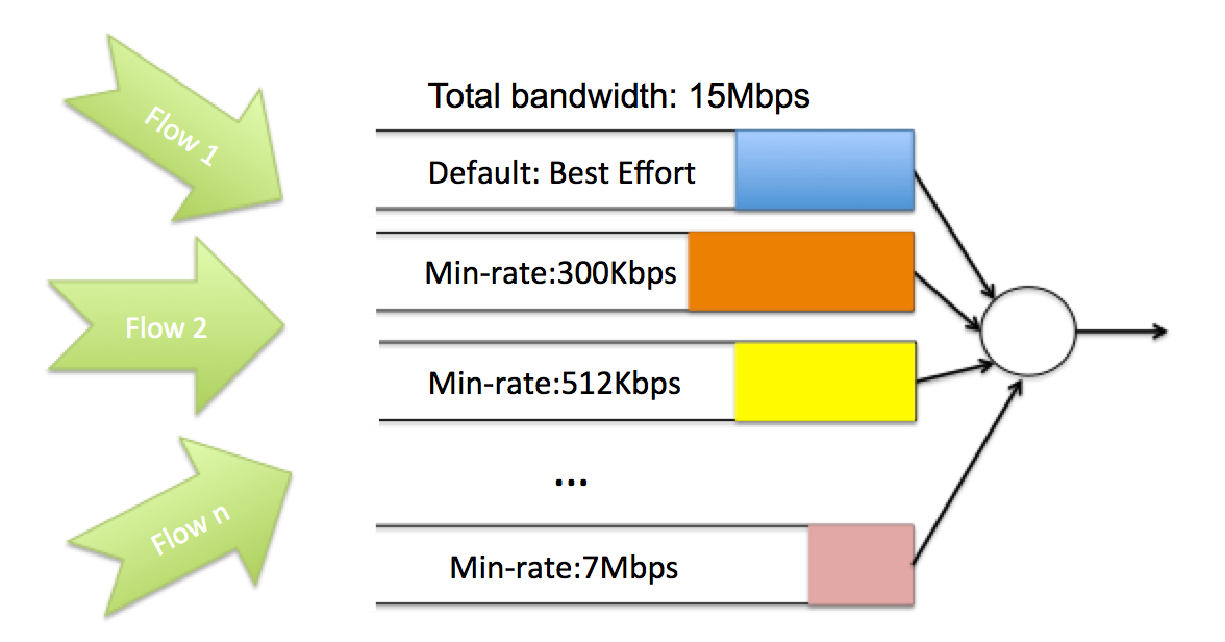
\includegraphics[width=0.5\textwidth]{assign_queue}
  \caption{}
  \label{fig:assign_queue}
\end{figure}

The control module is the core of QoSManager. The goal of the control module is to assign an appropriate rate to each flow so that
QoS of high priority applications can be effectively enforced. However, existing home routers do not support per-flow rate control
and even the Open vSwitch (OVS) does not yet support per-flow QoS described in OpenFlow 1.3 specification\todo{citation}. To overcome this limitation,
QosManager enables per-flow rate control by creating a list of queues with different sending rates at the ports of the shared link
\footnote{Here we assume that all the flows share a single link as shown in ~\reffig{setup}}. As shown in \reffig{assign_queue},
suppose the link capacity of the share link is \emph{C}, for each distinct bandwidth \emph{B} in the QoS configuration file,
we create $ N = \lfloor C / B \rfloor $ queues with minimal rate B and maximal rate C. In addition, we create a special queue $q_0$
only with maximal rate C. At runtime, QoSManager will assign each flow to a queue with an appropriate rate to control the rate of the
flow. Any flow that can not be guaranteed any level of QoS, it will be directly assigned to $q_0$.

To achieve the goal of the control module, we define the QoS utility function (\refsect{qosUF}) and propose a queue assignment
algorithm (\refsect{queueAssignAlgo}) to maximize the function under the limited link capacity.

\subsubsection{QoS Utility Function}
\label{sect:qosUF}
If the total bandwidth required by all the flows through a link exceeds the link capacity, it is obvious that the QoS requirements for
all the flows can not be fully satisfied and we need to somehow prioritize the applications' traffic flows. In order to quantify the QoS
requirements satisfied, we assign a score to each flow. The score function for a flow \emph{f} is defined as:
\begin{equation}
\scalebox{0.9}{
  $score(f) =
    \begin{cases}
      priority       & \quad \text{if } bw(f) = \text{ recommended}\\
      0.6 * priority & \quad \text{if } bw(f) = \text{ minimum}\\
      0              & \quad \text{if } \text{otherwise}\\
    \end{cases}$
}
\end{equation}

The score function basically says that if a flow can not be guaranteed any level of QoS, it gets 0 point. To distinguish between different
levels of QoS, we give full score to a flow if it is given recommended bandwidth and partial score to a flow if it is given minimum bandwidth.
We directly use priority as score. Therefore, higher priority application flow will get higher score if it is satisfied. Based on the score
function, the goal is to maximize the QoS utility function given a shared link with the capacity \emph{C}:

\begin{equation}
\begin{split}
  U_{QoS} = \sum_{i=1}^{n} score(f_i) \\ 
  \text{under } \sum_{i=1}^{n} bandwidth(f_i) \leq C
\end{split}
\end{equation}

It is clear that high priority application flows are more likely to be assigned their recommend bandwidth \emph{all the time} and the QoS of low
priority flows may be sacrificed. Moreover, the bandwidth allocated to high priority application will not be affected by new low priority flows
going through the link. It is possible that the total score of some lower priority flows is greater than the score of a high priority flow and
they cost less bandwidth. In that case, the bandwidth allocated to the high priority flow will be degraded. However, users can always tune the
priority at runtime to avoid this problem.

\subsubsection{Queue Assignment Algorithm}
\label{sect:queueAssignAlgo}

The optimization of the QoS utility function is very similar to the Knapsack problem \todo{citation} which can be effectively solved by dynamic
programming. However, our problem differs form the canonical bounded knapsack problem in two ways. First, in our settings, an "object" (flow) has
two "values" (full and partial score) and two corresponding "volumes" (recommended and minimal bandwidth). You can only choose one of them to put
into the "knapsack" (shared link). Second, in order to avoid fluctuation, we want to keep a flow in the same queue as long as possible. That being
said, when new objects come and we need to reorganize the knapsack, we want to keep as many old objects in the knapsack as possible. What's more,
since the knapsack is usually much larger than the smallest object, it is not memory efficient to use the dynamic programming. Instead, we use
depth-first search (~\refalg{queueAssignAlgo}) to search for the optimal assignment.

\begin{algorithm}
  \SetKwData{X}{x} \SetKwData{Timestamp}{timestamp} \SetKwData{Priority}{priority}
  \SetKwFunction{Sort}{Sort}
  \SetKwInOut{Input}{input}
  \SetKwInOut{Output}{output}

  \Input{A List $flowList$}
  \Output{A Map $assign$}
  
  \Sort($flowList$, key=$\lambda$ \X: \X.\Timestamp)\;
  \Sort($flowList$, key=$\lambda$ \X: \X.\Priority, reverse);



  \caption{Queue Assignment Algorithm}\label{alg:queueAssignAlgo}
\end{algorithm}

The algorithm takes a list \emph{flowList} and the shared link capacity \emph{C} as input. The \emph{flowList} merges the tc\_table and the
QoS configuration. We assume that all the flows in the \emph{flowList} are successfully classified by the traffic classification module. If a flow
can not be recognized by the traffic classification module, it will be directly assigned to $q_0$. The algorithm first sort the \emph{flowList} by
timestamp and then by priority. Assume that the sorting algorithm is table, and then we will always pick the flows in a "first come first serve" manner
if there are multiple flows of the same application type. Then the algorithm invokes depth-first search procedure to search for the optimal assignment.

\section{Evaluation}
\label{sect:experiment}
\subsection{Evaluation setup}
Mininet
\subsubsection{Scenario 1}
Generate traffic for different services at the same time

\subsubsection{Scenario 2}
Generate traffic for one service first, then generate other traffic later  




\section{Conclusion and Future work}
\label{sect:future}

In this paper, we have presented QoSManager, a configurable and adaptive QoS management framework
based on SDN. Users specify high-level QoS policies through a web interface and QoSManager controller
will dynamically assign each flow to a queue with an appropriate rate. We take into account the fact
that an application may have different levels of QoS requirements in different scenarios and provide
users with great flexibility to define their policies. In the experiment, we have demonstrated that
the shared bandwidth is allocated in the way that the QoS of high priority applications are effectively
enforced.

We focused on the control module in this paper and left other modules in the framework quite simple.
The next step in our work is to improve these modules. For instance, the traffic classification module
uses a statically defined database to perform the classification. We plan to adopt machine learning
approach \todo{citation see traffic survey paper} to perform more sophisticated classification. The forwarding module now simply implements a L2
switch. We are thinking of introducing QoS based routing \cite{Apostolopoulos_SIGCOMM98, Egilmez_ASPIPA12}
into the module. In addition, we are planning to provide more flexibility for users to define time-based
QoS and device-based QoS.


\newpage
% references section
\bibliographystyle{plain}
\bibliography{ref/ref}

\end{document}
